% Options for packages loaded elsewhere
\PassOptionsToPackage{unicode}{hyperref}
\PassOptionsToPackage{hyphens}{url}
%
\documentclass[
]{article}
\usepackage{lmodern}
\usepackage{amssymb,amsmath}
\usepackage{ifxetex,ifluatex}
\ifnum 0\ifxetex 1\fi\ifluatex 1\fi=0 % if pdftex
  \usepackage[T1]{fontenc}
  \usepackage[utf8]{inputenc}
  \usepackage{textcomp} % provide euro and other symbols
\else % if luatex or xetex
  \usepackage{unicode-math}
  \defaultfontfeatures{Scale=MatchLowercase}
  \defaultfontfeatures[\rmfamily]{Ligatures=TeX,Scale=1}
\fi
% Use upquote if available, for straight quotes in verbatim environments
\IfFileExists{upquote.sty}{\usepackage{upquote}}{}
\IfFileExists{microtype.sty}{% use microtype if available
  \usepackage[]{microtype}
  \UseMicrotypeSet[protrusion]{basicmath} % disable protrusion for tt fonts
}{}
\makeatletter
\@ifundefined{KOMAClassName}{% if non-KOMA class
  \IfFileExists{parskip.sty}{%
    \usepackage{parskip}
  }{% else
    \setlength{\parindent}{0pt}
    \setlength{\parskip}{6pt plus 2pt minus 1pt}}
}{% if KOMA class
  \KOMAoptions{parskip=half}}
\makeatother
\usepackage{xcolor}
\IfFileExists{xurl.sty}{\usepackage{xurl}}{} % add URL line breaks if available
\IfFileExists{bookmark.sty}{\usepackage{bookmark}}{\usepackage{hyperref}}
\hypersetup{
  pdftitle={Some exploration of Oxford Policy Response Database},
  pdfauthor={Lio},
  hidelinks,
  pdfcreator={LaTeX via pandoc}}
\urlstyle{same} % disable monospaced font for URLs
\usepackage[margin=1in]{geometry}
\usepackage{graphicx,grffile}
\makeatletter
\def\maxwidth{\ifdim\Gin@nat@width>\linewidth\linewidth\else\Gin@nat@width\fi}
\def\maxheight{\ifdim\Gin@nat@height>\textheight\textheight\else\Gin@nat@height\fi}
\makeatother
% Scale images if necessary, so that they will not overflow the page
% margins by default, and it is still possible to overwrite the defaults
% using explicit options in \includegraphics[width, height, ...]{}
\setkeys{Gin}{width=\maxwidth,height=\maxheight,keepaspectratio}
% Set default figure placement to htbp
\makeatletter
\def\fps@figure{htbp}
\makeatother
\setlength{\emergencystretch}{3em} % prevent overfull lines
\providecommand{\tightlist}{%
  \setlength{\itemsep}{0pt}\setlength{\parskip}{0pt}}
\setcounter{secnumdepth}{-\maxdimen} % remove section numbering

\title{Some exploration of Oxford Policy Response Database}
\author{Lio}
\date{21/05/2020}

\begin{document}
\maketitle

\hypertarget{comparison-with-coronanet}{%
\subsection{Comparison with CoronaNet}\label{comparison-with-coronanet}}

Simply plotting all observations from CoronaNet (CN) and the Oxford
Database (Ox) reveals that, as expected, both are quite correlated
(0.7), but the relationship is far from being perfect.

\begin{verbatim}
## `geom_smooth()` using formula 'y ~ x'
\end{verbatim}

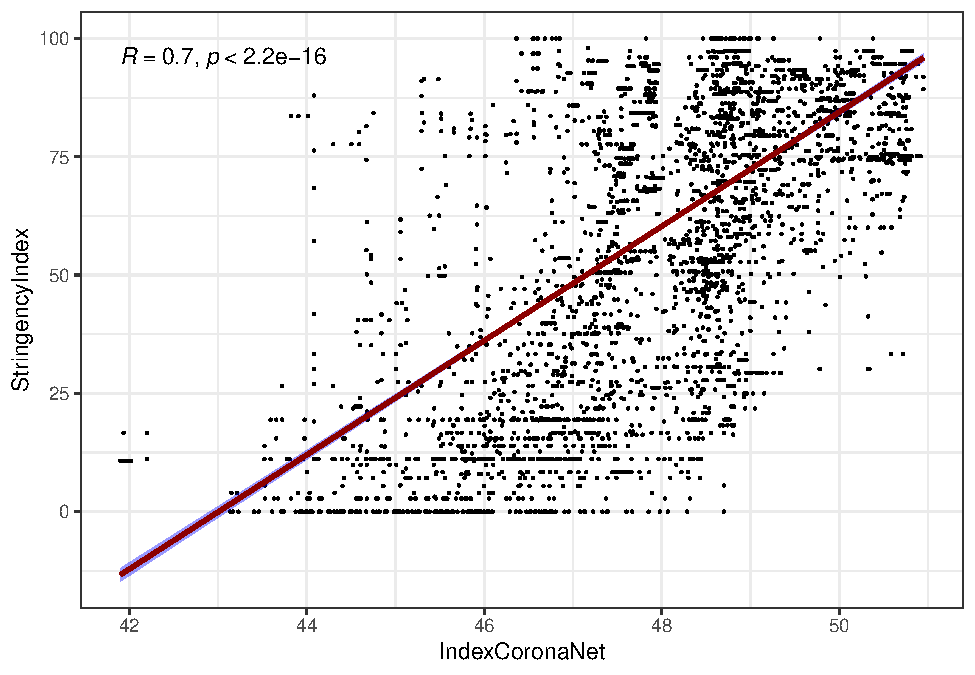
\includegraphics{LR_explore_files/figure-latex/scatter-1.pdf}

Illustrating this for a couple of (partly random) countries further
shows where these differences stem from. A couple of things:

\begin{itemize}
\tightlist
\item
  CN starts at random periods, and often with odd values (suggesting
  quite strict policies at points in time where most likely no measures
  had been taken)
\item
  CN doesn't exhibit a line for US here, because it is federal and they
  report by state. Ox do the aggregation for us, whether this is to our
  satisfaction will have to be seen.
\item
  Easing of lockdowns seems to be hardly reflected in CN data, whereas
  Ox seems quite responsive.
\end{itemize}

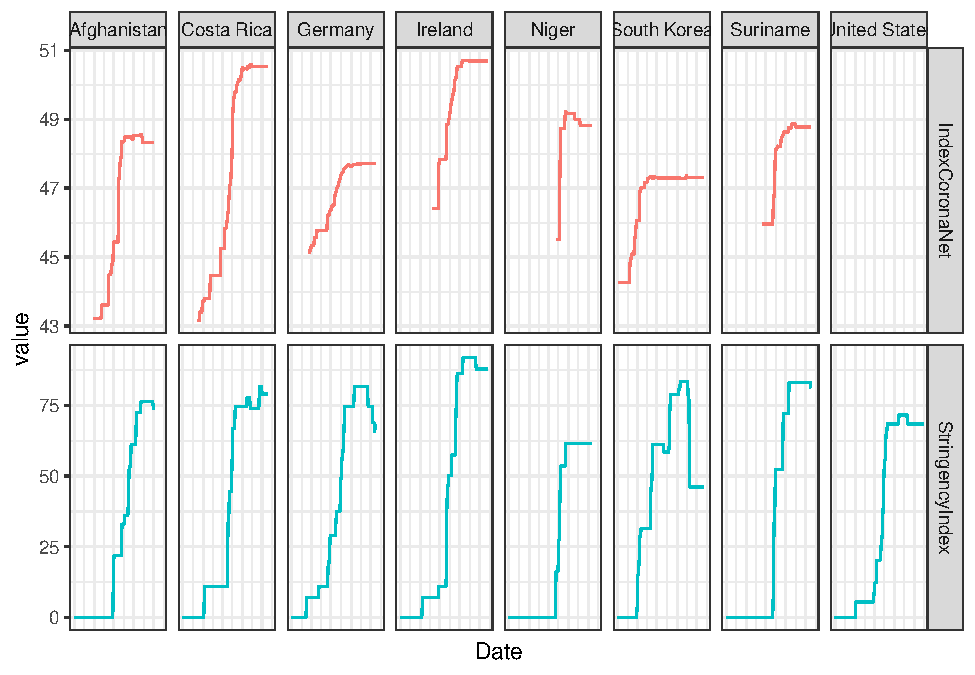
\includegraphics{LR_explore_files/figure-latex/lines compare-1.pdf}

Overall, it feels safe to assume that Ox is the better dataset to work
with.

\hypertarget{plotting-duration-of-individual-measures}{%
\subsection{Plotting duration of individual
measures}\label{plotting-duration-of-individual-measures}}

Ox comes with the neat `flag' variables, which are 1 if any given
measure is in place and 0 otherwise (there is also the version that
ranges 0-3 and says something about intensity).

The graph below is an attempt at depicting that information in a single
graph, admittedly implemented in a slightly overcomplicated way
(somewhat cheating ggplot)). The information content is quite high I
find, I just wish I'd gone for a simpler approach (e.g.~seperate graphs
for index and measures, line chart on top and bar chart / gantt chart
below for each country). Also, that's why the legend is improvised.

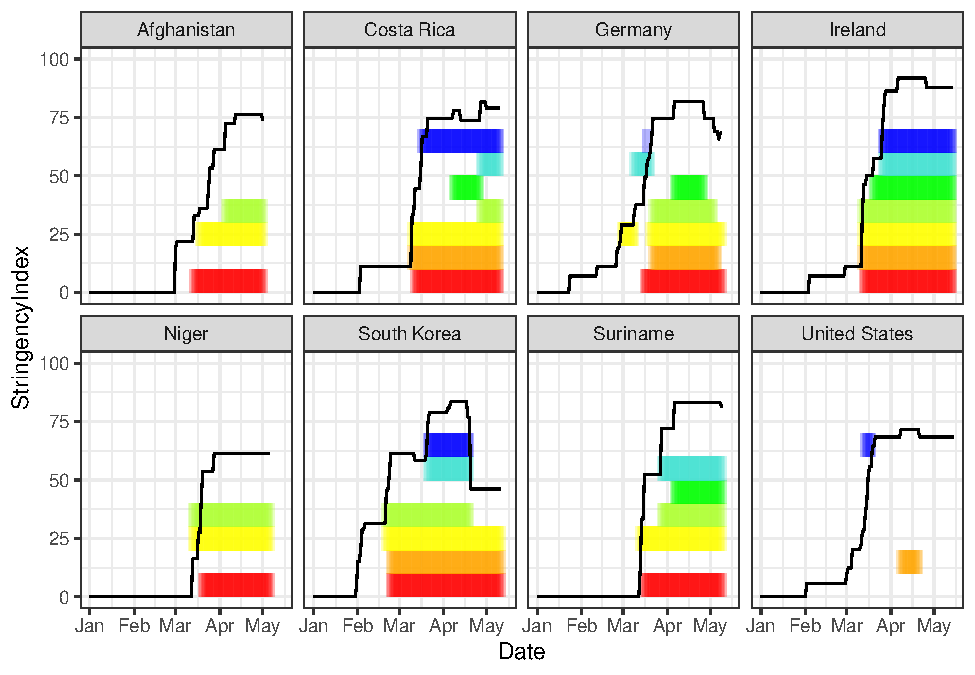
\includegraphics{LR_explore_files/figure-latex/measures-1.pdf}

\end{document}
